\part{Data Analysis and Dislaying}
\section{Analysis of the data}
Total implementation link for data analyzer : \\
\url{https://github.com/Sprea22/Data_Analyzer_Python}

During this part the main purpose is to analyze the whole dataset in order to find some kind of useful informations later on. 

The output of this phase will basically be for each single data input:
\begin{itemize}
\item Total graphic of the input data from 2005 to 2016.
\item Graphic of the input data for each single year from 2005 to 2016.
\item Correlation matrix between different months of the same input.
\item Correlation matrix between different years of the same input.
\end{itemize}

And then it also provides:
\begin{itemize}
\item General correlation matrix between all the different inputs.
\item Graphic of the normalized angular coefficients of all the inputs.
\end{itemize}

It's important to remind that this phase can be implemented in different ways and with different programming language;\\
This proceure will describes the system implentation using Python, so be sure to have installed all the necessary for compile and execute Python code on your platform.

Current development environment:\\
Python version: 2.7.12\\
Linux kernel version number: Linux Asus 4.4.0-71-generic SMP\\

The system that it's going to be implemented during this part of the work could be divided in two subsystems:
\begin{itemize}
\item Single Input Analyzer (SIA): Used for analyze a single data input.
\item Multiple Inputs Analyzer (MIA): Used for analyze multiple data inputs.
\end{itemize}
\newpage


\newpage
\subsection{Single Input Analyzer}
It's possible to check out the total implementation code of the SIA in the appendice  [\ref{SIA_Implementation}].
The implementation of this Analyzer can be divided in the following parts:
\begin{itemize}
\item SIA imported libraries. 
\item SIA part I: Generate and display a graphic about current input with total data from 2005 to 2016.
\item SIA part II: Generate and display a graphic about current input for each year from 2005 to 2016.
\item SIA part III: Generate and display a graphic that contains the correlation matrix between each single year from 2005 to 2016 of the current input.
\item SIA part IV: Generate and display a graphic that contains the correlation matrix between each single months of the year of the current input.
\item SIA part V: Generate and display a single overview image for the current input.
\end{itemize}

\subsubsection{SIA: Requirements for reusability}
The system that is going to be implemented in this phase of the work could be used for other data inputs as well, but there are of course some kind of requiriments about the dataset that are necessary for let it works in a proper way.\\
The aalysis system need in input a dataset structure that:
\begin{itemize}
\item Data from January 2005 to December 2016
\item One single value for each month
\end{itemize}
It means that the dataset must contains 144 values for each single input.

\subsubsection{SIA: Imported libraries}
Specific Python libraries have been imported for the implementation of this system.
It's possible to find out a list of this libraries with a specific description for each of them in the appendice [\ref{SIA_libraries}].

\newpage

\subsubsection{SIA section I: Total graphic for all the years}
\textbf{Goal:}\\
Generate and display the total graphic about current input from 2005 to 2016.

\textbf{Requirements:}\\
- Data content: 144 values, 1 value for each month from 2005 to 2016

\textbf{Implementation:}\\
It's possible to check out the full ccommented code in the appendice: [\ref{SIA_section_I}]

\textbf{Results:} \\
With this first part of the code has been reached the first goal of displaying and saving the basic graphic about the current input from 2005 to 2016 with also the relative trendline, that looks like this example:

\begin{figure}[H]
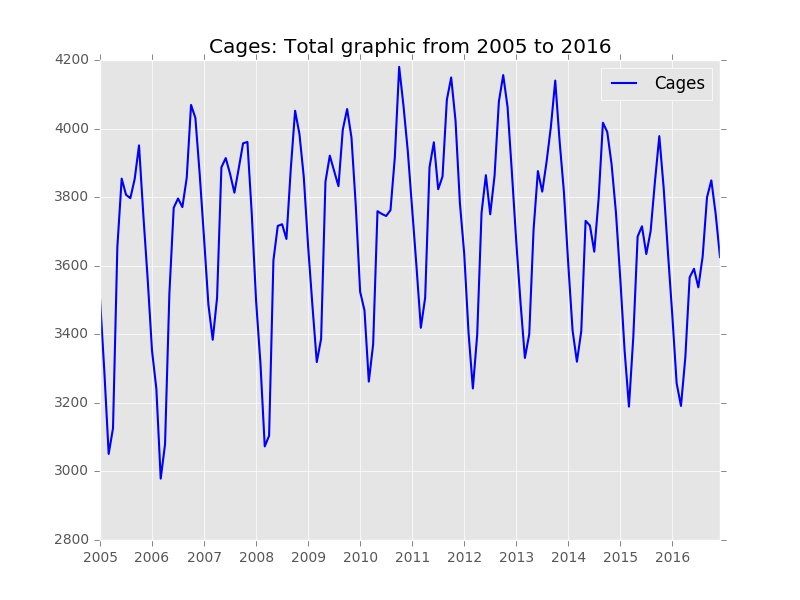
\includegraphics[width=1\textwidth]{Files/Cages_Total.jpg}
\caption{Total graphic about current input with total data from 2005 to 2016.}
\end{figure}



\newpage
\subsubsection{SIA section II: Single graphics for each year}

\textbf{Goal:}\\
Generate and display a graphic that contains the plots of each single year from 2005 to 2016 of the current input. 

\textbf{Requirements:}\\
- Data content: 144 values, 1 value for each month from 2005 to 2016

\textbf{Implementation:}\\
It's possible to check out the full ccommented code in the appendice: [\ref{SIA_section_II}]

\textbf{Results:} \\
With this second part of the code has been reached the goal of displaying and saving the graphic of the plots for each single year of the current input from 2005 to 2016, that looks like this example:

\begin{figure}[H]
	\centering
    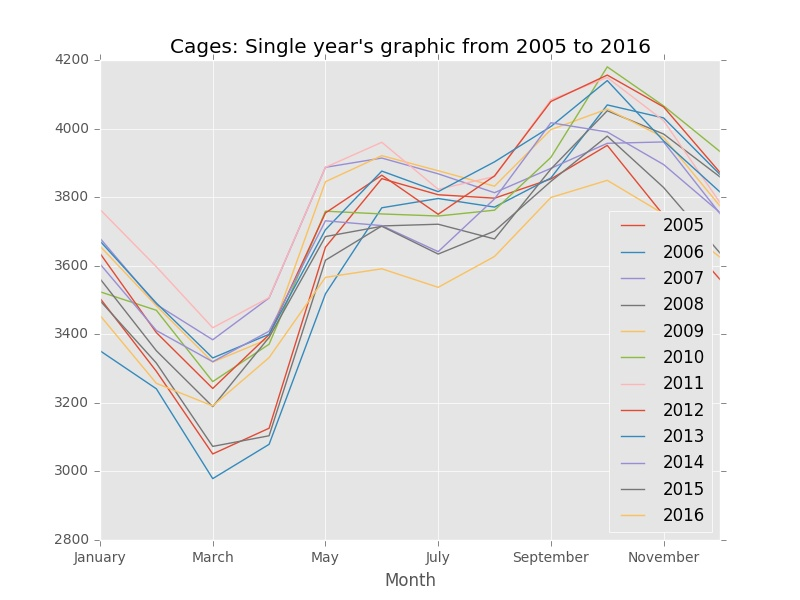
\includegraphics[width=1\textwidth]{Files/Cages_Years.jpg}
    \caption{Graphics for each single year of the input data from 2005 to 2016}
\end{figure}




\newpage
\subsubsection{SIA section III: Correlation matrix between years}

\textbf{Goal:}\\
Calculate the correlation coefficients between each single year from 2005 to 2016 of the current input and then display it with a correlation matrix.

\textbf{Requirements:}\\
- Data content: 144 values, 1 value for each month from 2005 to 2016

\textbf{Implementation:}\\
It's possible to check out the full ccommented code in the appendice: [\ref{SIA_section_III}]

\textbf{Results:} \\
With this part of the code have been calculated the correlation coefficients between each single year from 2005 to 2016 of the current input and saved it in a document. \\
Then has been also displayed and saved the correlation matrix about it, that looks like the current example:

\begin{figure}[H]
	\centering
    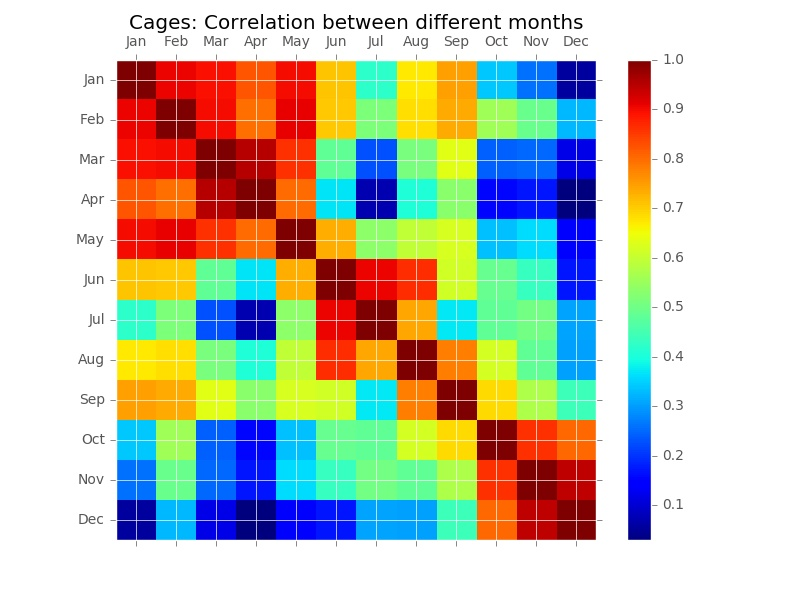
\includegraphics[width=1\textwidth]{Files/Cages_Months_Matrix.jpg}
    \caption{Correlation matrix between different months of the same input}
\end{figure}




\newpage
\subsubsection{SIA section IV: Correlation matrix between months}

\textbf{Goal:}\\
Calculate the correlation coefficients between each single month from 2005 to 2016 of the current input and then display it with a correlation matrix.

\textbf{Requirements:}\\
- Data content: 144 values, 1 value for each month from 2005 to 2016

\textbf{Implementation:}\\
It's possible to check out the full ccommented code in the appendice: [\ref{SIA_section_IV}]


\textbf{Results:} \\
With this part of the code have been calculated the correlation coefficients between each single month from 2005 to 2016 of the current input and saved it in a document. \\
Then has been also displayed and saved the correlation matrix about it, that looks like the current example:

\begin{figure}[H]
	\centering
    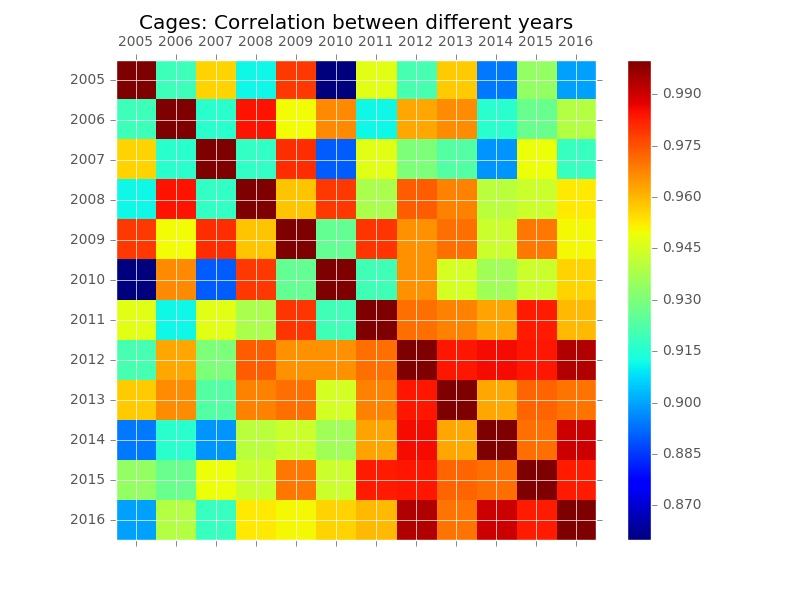
\includegraphics[width=1\textwidth]{Files/Cages_Years_Matrix.jpg}
    \caption{Correlation matrix between different years of the same input}
\end{figure}


\newpage
\subsubsection{SIA section V: Single overview}

\textbf{Goal:}\\
Generate and display a single overview image that contains all the graphics previous calculated for the current input.

\textbf{Implementation:}\\
It's possible to check out the full ccommented code in the appendice: [\ref{SIA_section_V}]

\textbf{Requirements:}\\
- All the graphics about the current input have to be already calculated and saved.

\textbf{Results:}
With this part of the code it's possible to have a single overview image for the current input, that is basically showing and comparing all the graphics that have already been calculated about this input. It looks like this example:
\begin{figure}[H]
    \makebox[\textwidth][c]{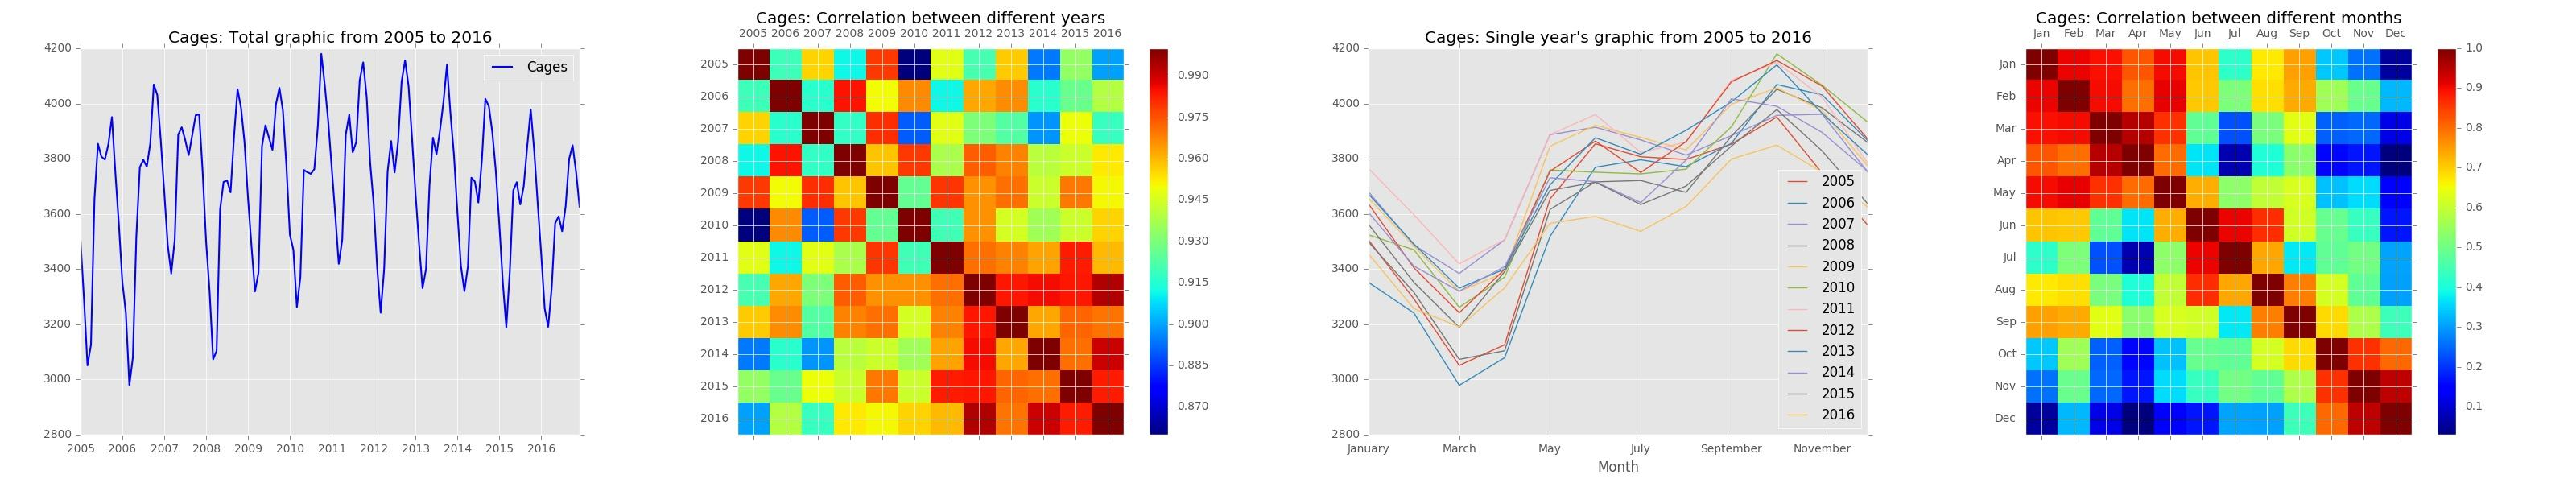
\includegraphics[width=1.4\textwidth]{Files/Cages_Overview.jpg}}
    \caption{Example of "Single Input Overview Image"}
\end{figure}

\newpage

\subsection{Multiple Inputs Analyzer}
\subsubsection{MIA: Requirements for reusability}
The system that is going to be implemented during this phase it's not reusable at all.
It means that has been implemented just for analyze and display the result about the dataset that is used during this work.

\subsubsection{SIA: Imported libraries}
Specific Python libraries have been imported for the implementation of this system.
It's possible to find out a list of this libraries with a specific description for each of them in the appendice [\ref{MIA_Libraries}].

\newpage

\subsubsection{MIA: Implementation}
\textbf{Goal:}\\
This analyzer is mainly used for show the correlation coefficent between the diffent inputs along the total period (from 2005 o 2016) and also for display the comparison between the normalized angular coefficients for each single input in the current dataset.

\textbf{Requirements:}\\
How it's written above, this part of the system is not reusable at all.\\
So the requirements are strict about the input data, that have to be exactly tha same that we are using during this work.\\
Of course this system can be used for the other dataset, but before doing it you have to personalize the implementation code.

\textbf{Implementation:}\\
It's possible to check out the full ccommented code in the appendice: [\ref{MIA_Implementation}]

\textbf{Results:} \\
The first part of the MIA implementation allows to calculate the correlation coefficients value between each single inputs and then also to display and save it. The graphic result looks like:

\begin{figure}[H]
	\centering
    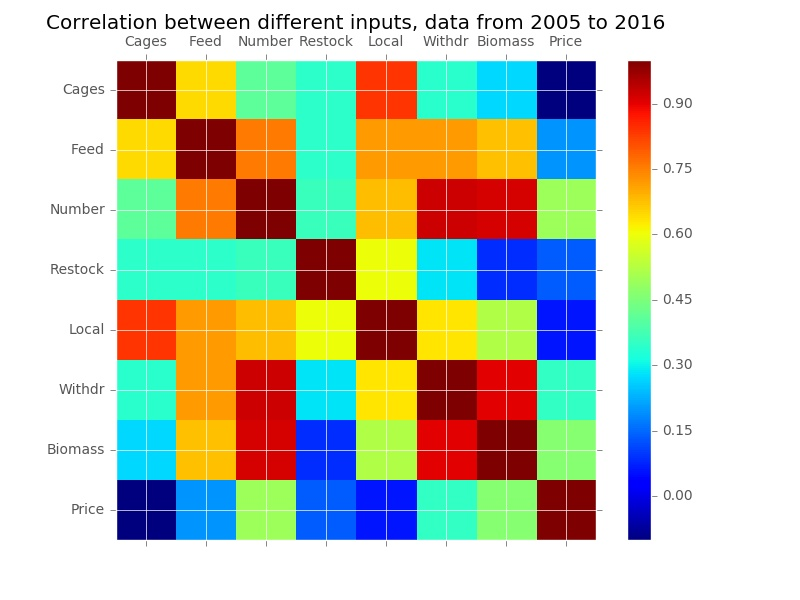
\includegraphics[width=0.90\textwidth]{Files/Total_Dataset_Years_Matrix.jpg}
    \caption{Correlation matrix between different inputs with data from 2005 to 2016.}
\end{figure}

\newpage

The second part of the MIA implementation allows to display a graphic that compare the normalized angular coefficients for each single input that have been already calculated and reported in a document. The result graphic look like:

\begin{figure}[H]
	\centering
    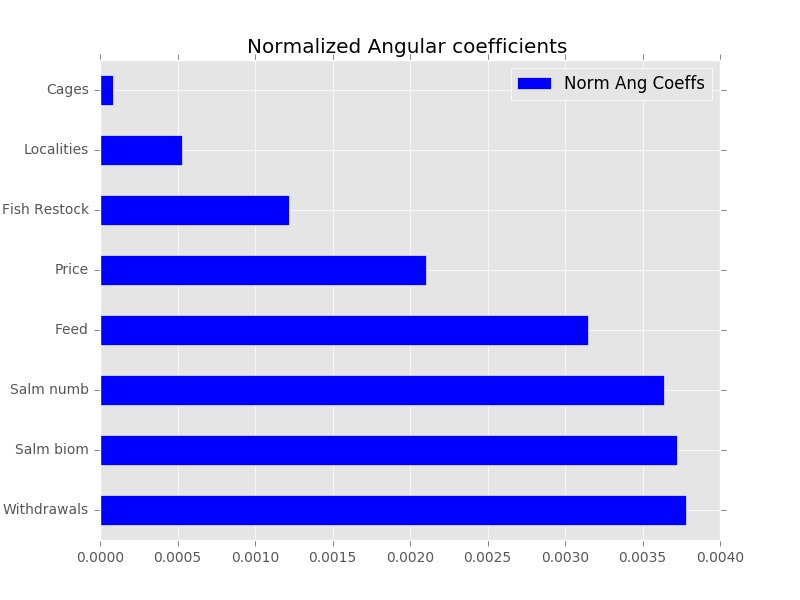
\includegraphics[width=0.90\textwidth]{Files/Norm_Ang_Coeffs.jpg}
    \caption{Normalized angular coefficients of each input's trendline.}
\end{figure}


\newpage
\section{Extract information from data}
